\chapter{Progettazione}
\section{Diagramma delle classi }
\begin{center}	
	\vspace{1ex}
	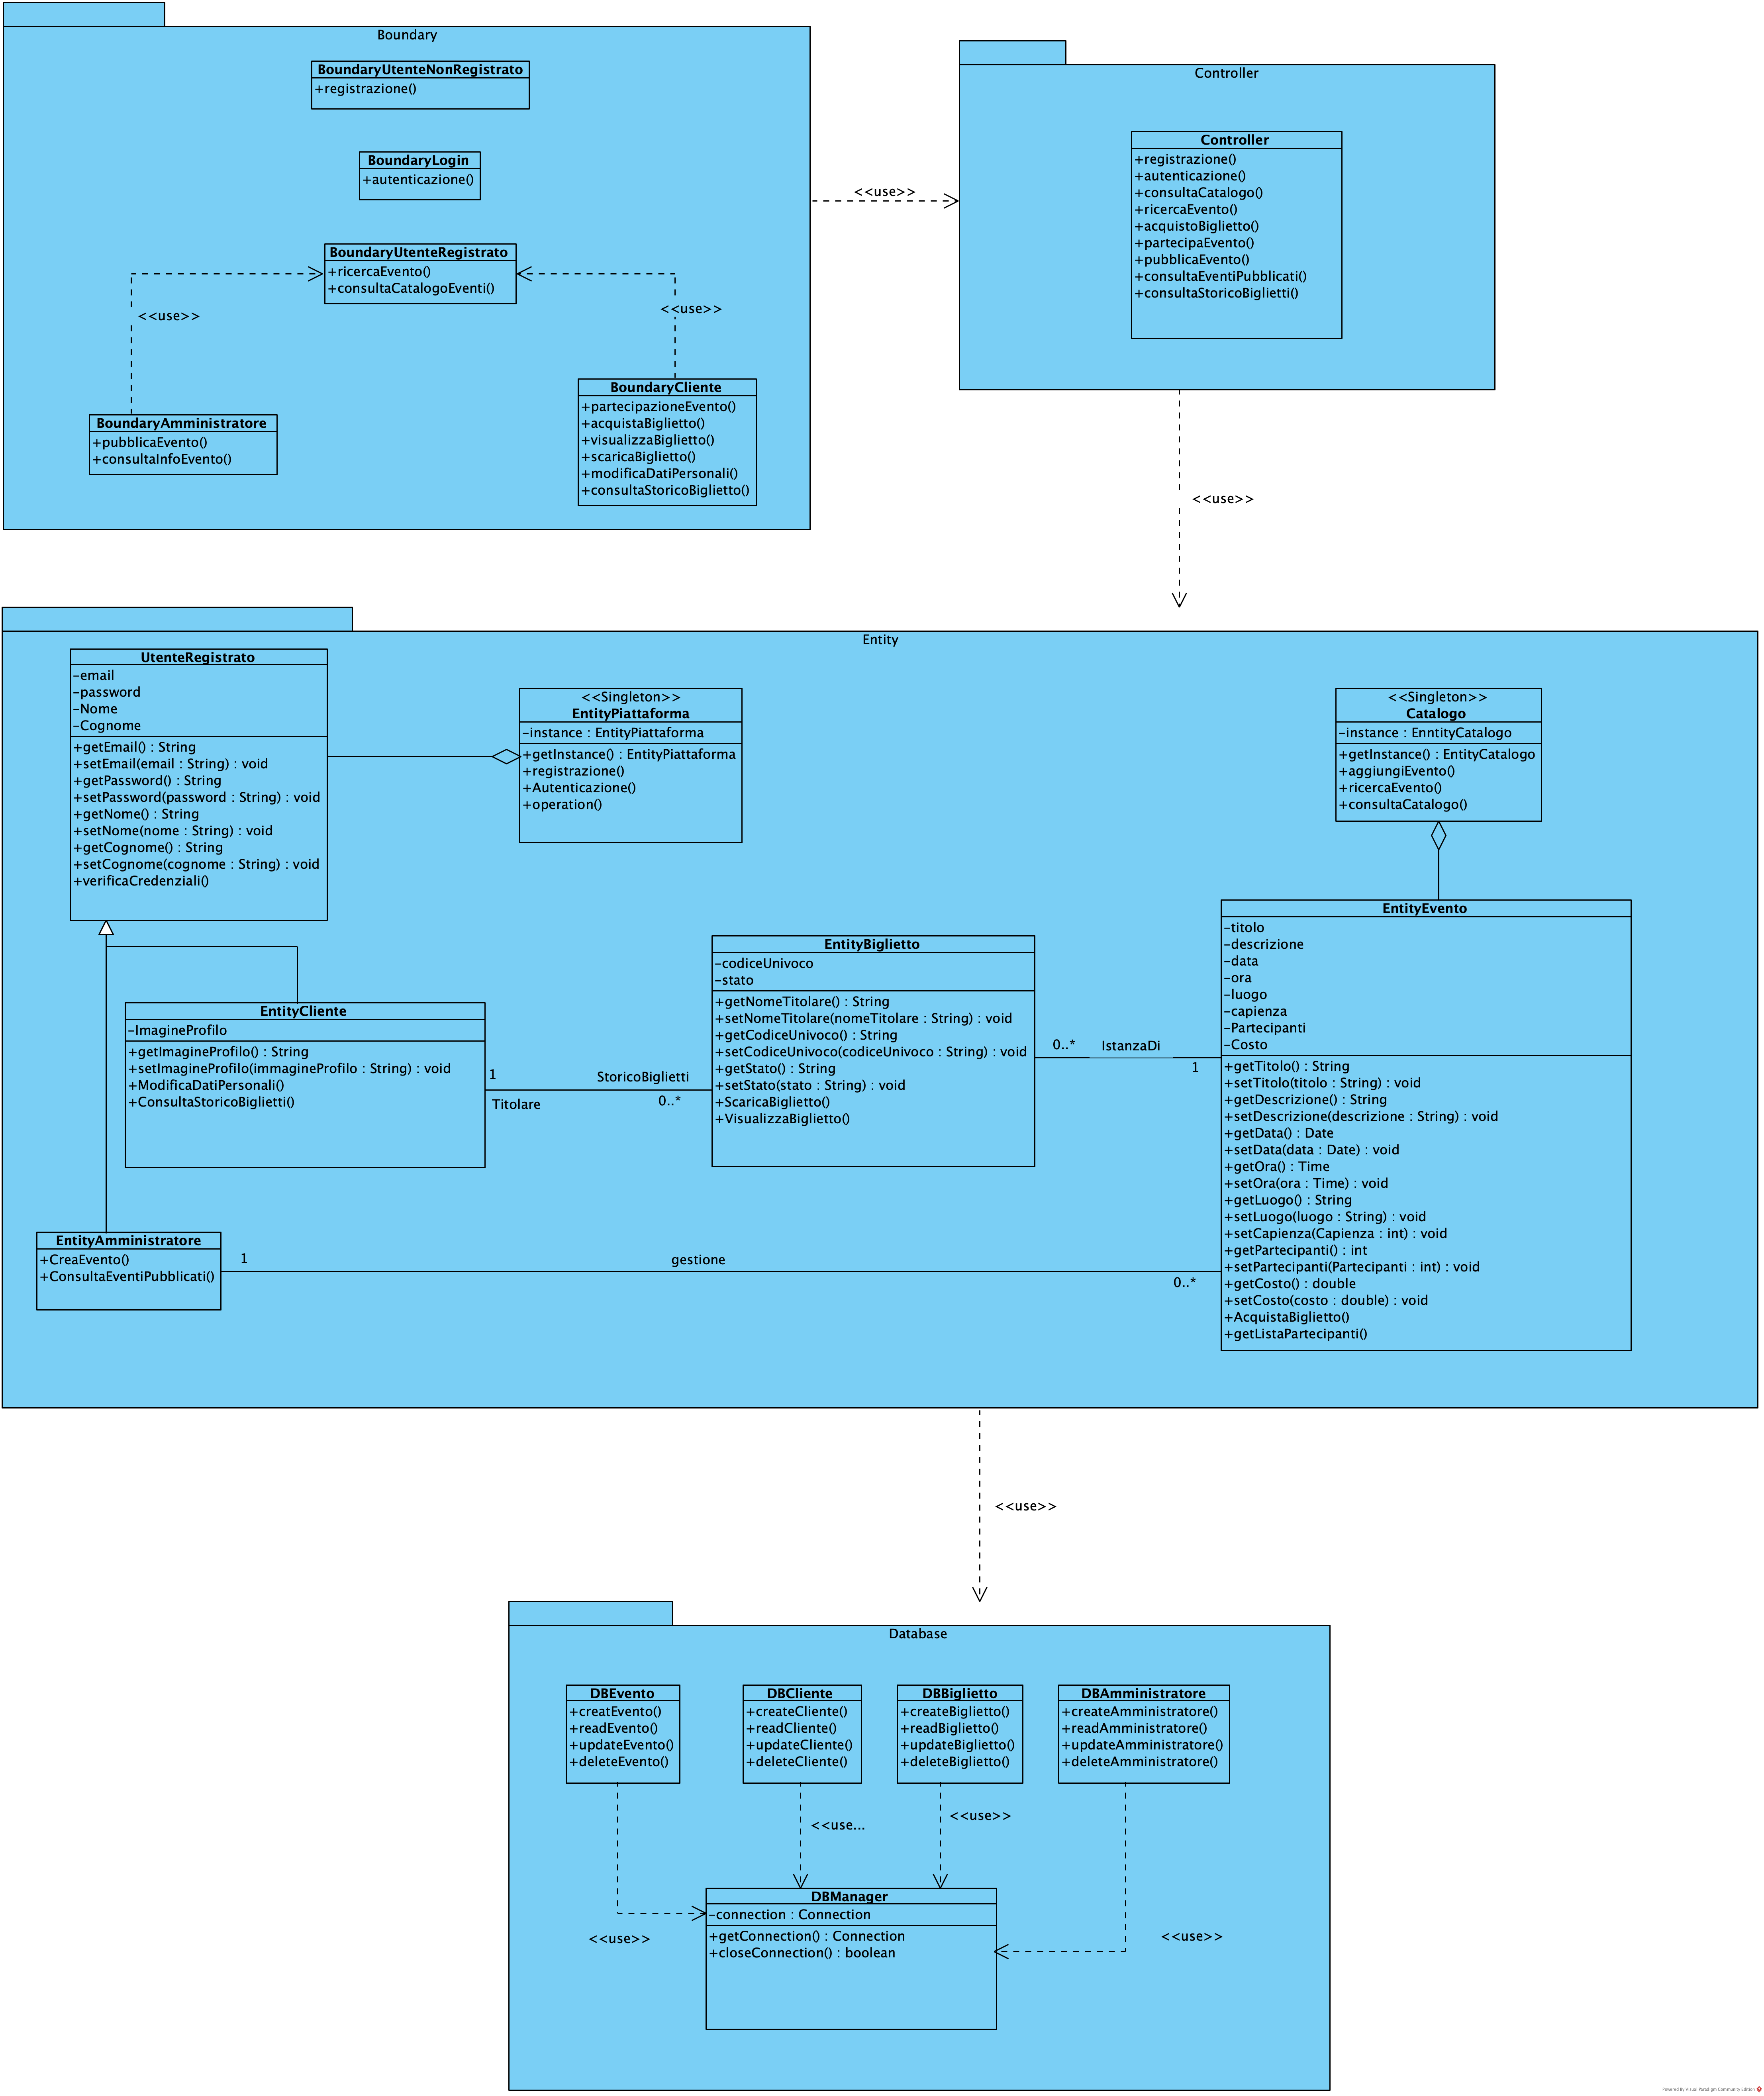
\includegraphics[height=0.9\linewidth]{assets/package/Diagrammadelleclassi.png}
	\vspace{1ex}
\end{center}
\subsection{Package Entity}
\begin{center}	
	\vspace{1ex}
	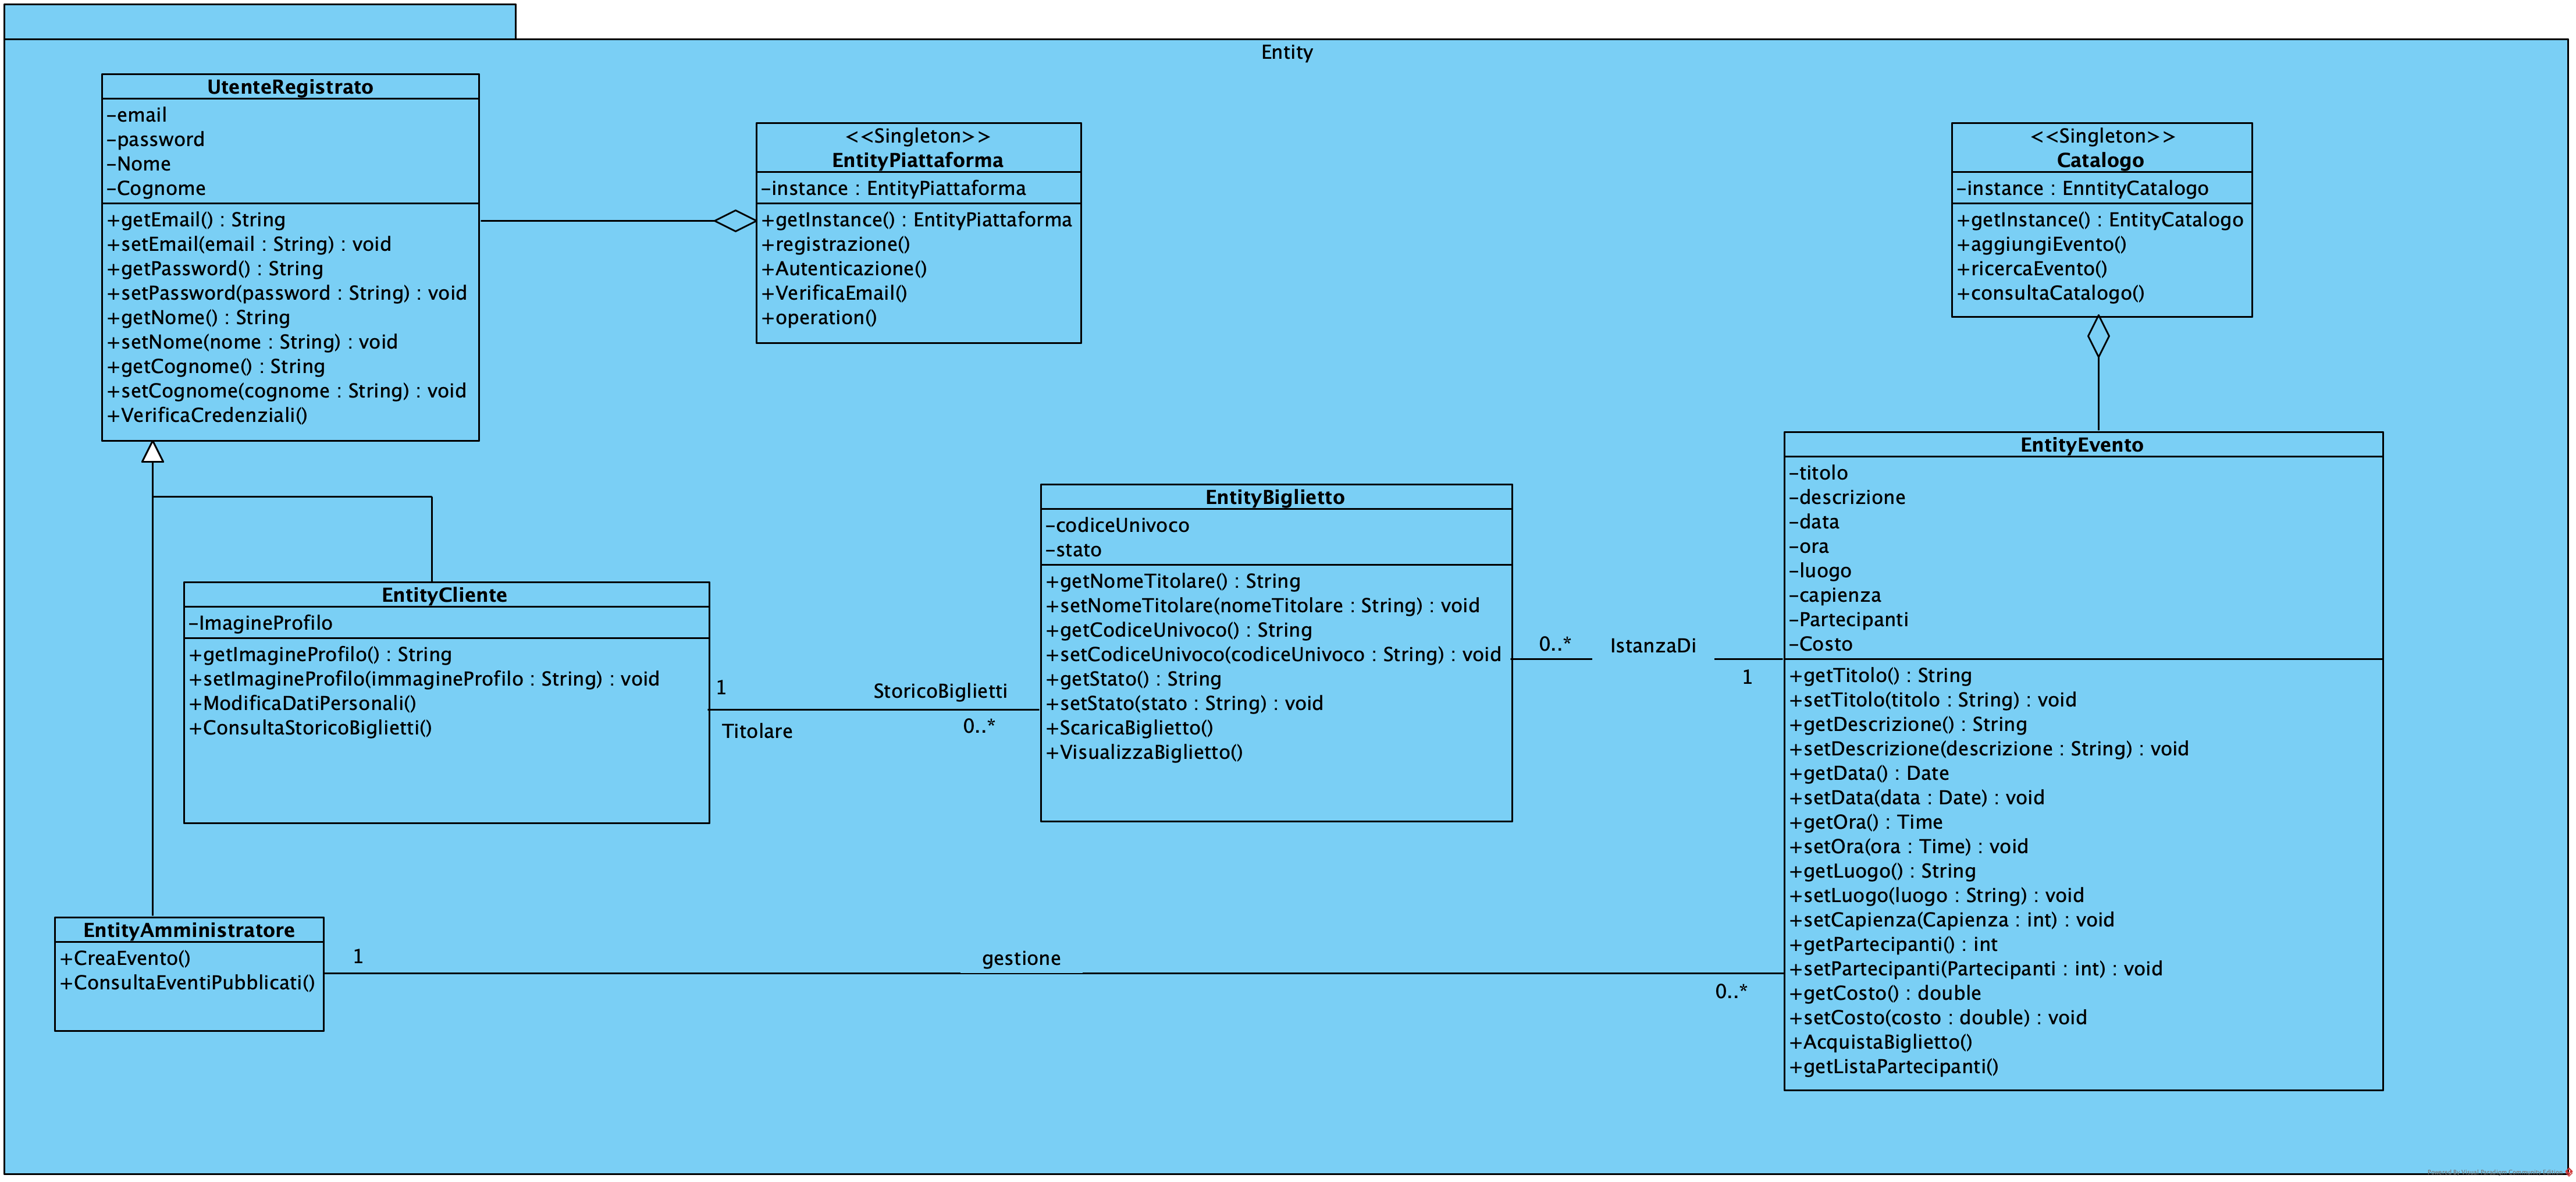
\includegraphics[height=0.38\linewidth]{assets/package/entity.png}
	\vspace{1ex}
\end{center}
\subsection{Package Boundary}
\begin{center}	
	\vspace{1ex}
	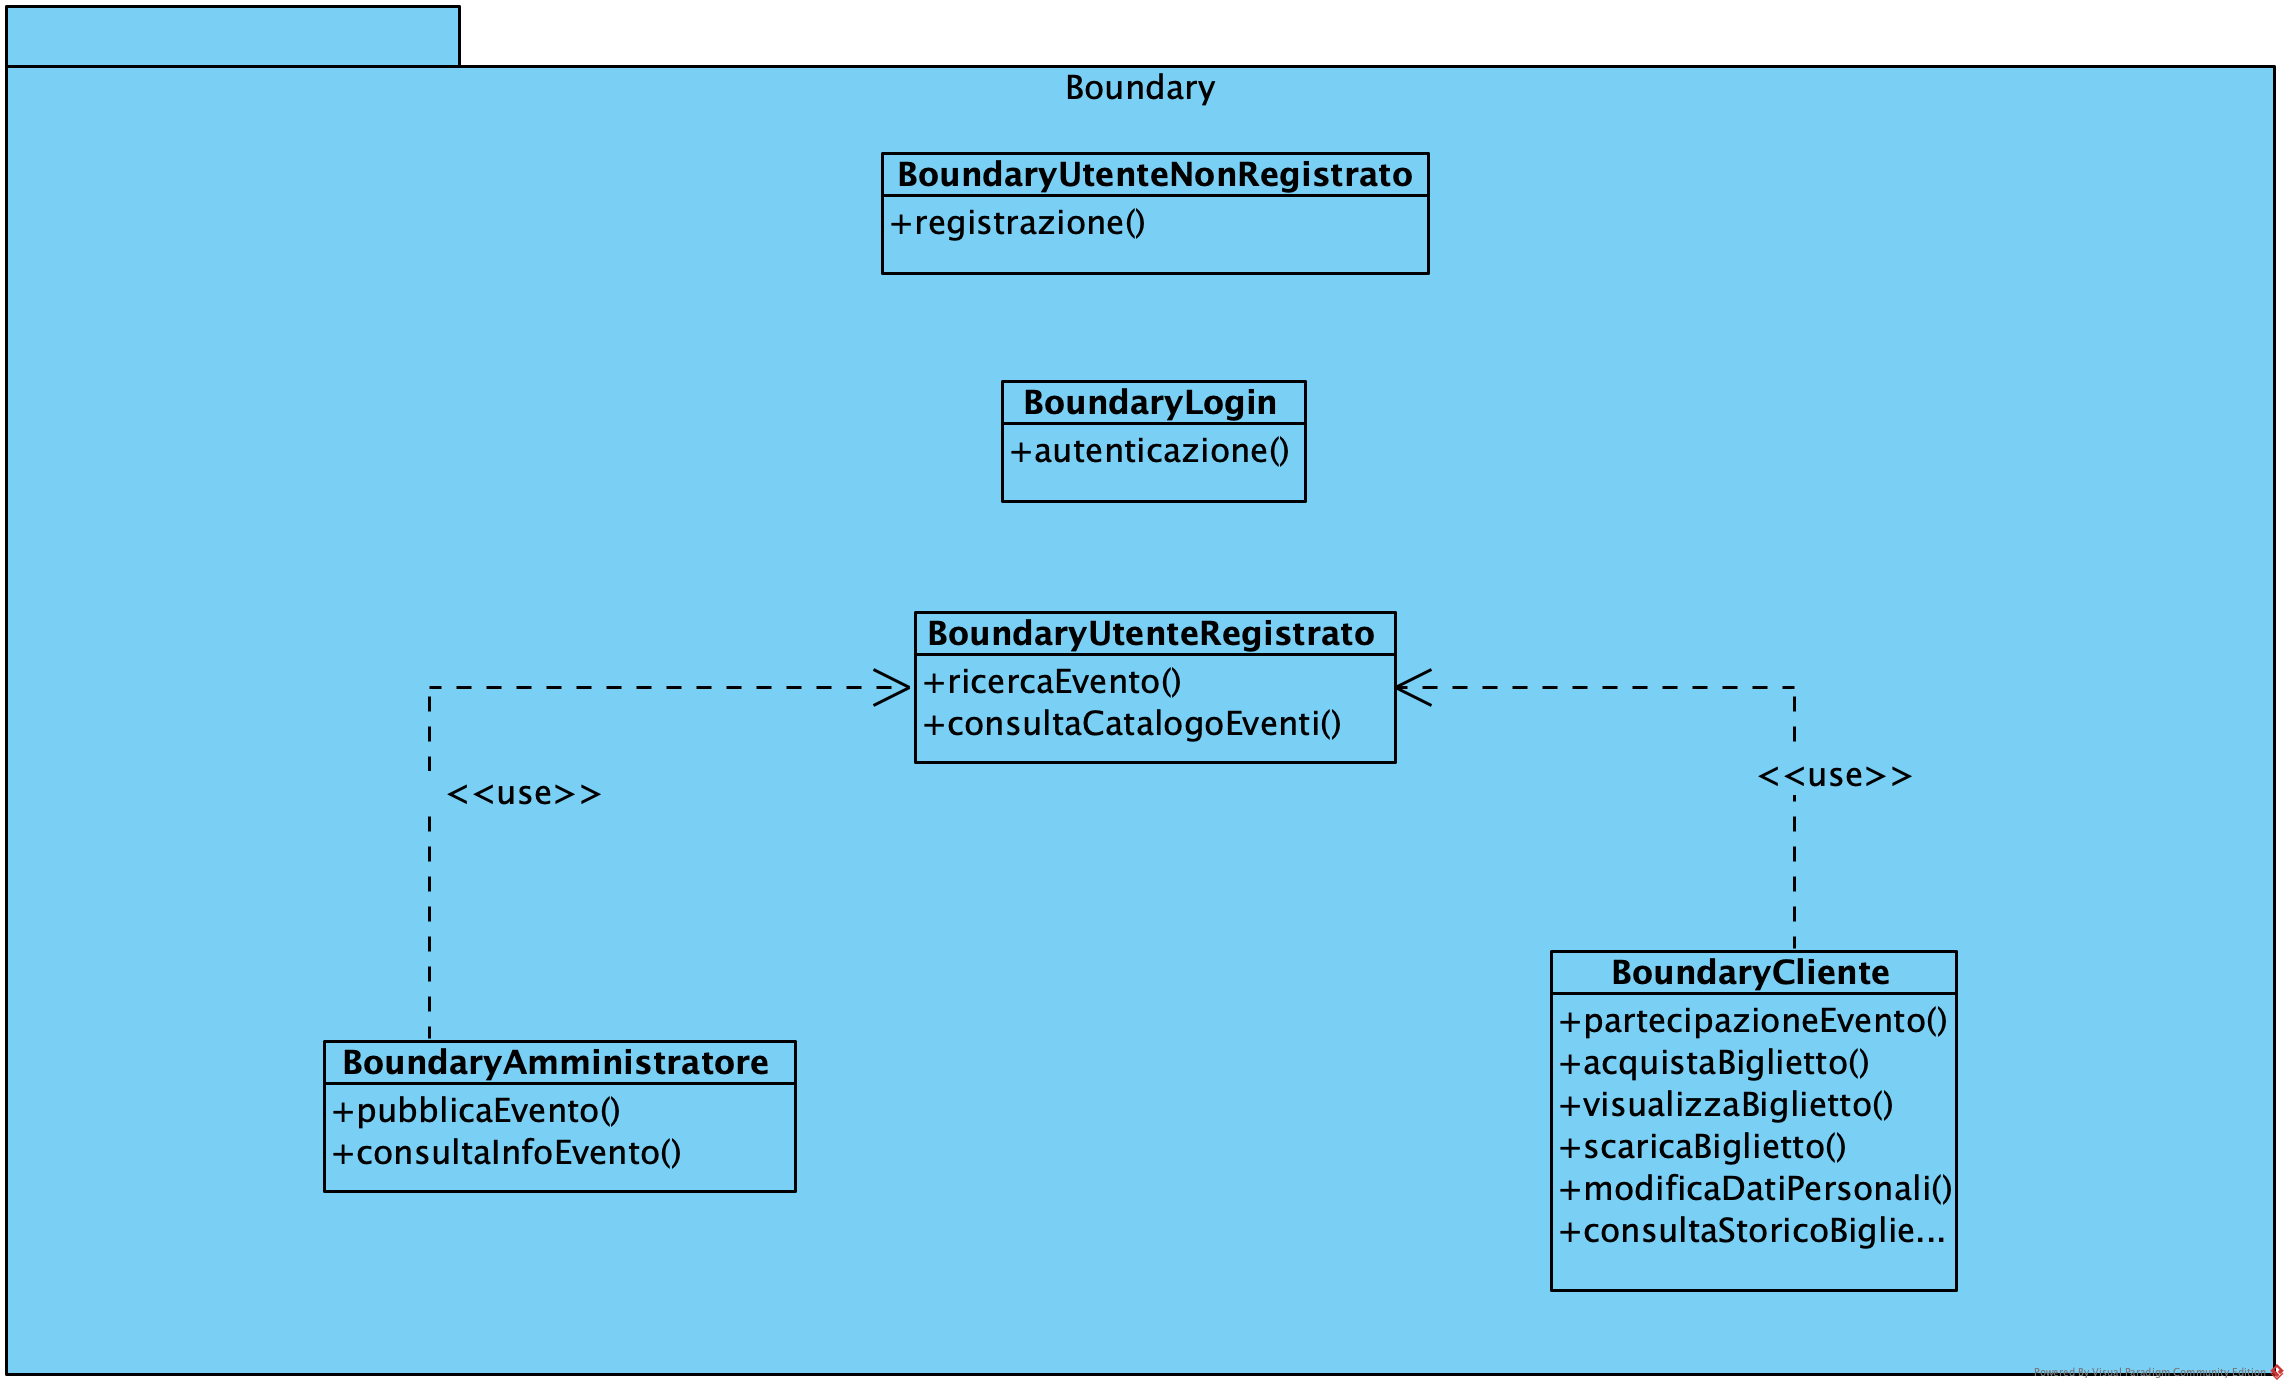
\includegraphics[height=0.38\linewidth]{assets/package/Boundary.png}
	\vspace{1ex}
\end{center}
\subsection{Package Controller}
\begin{center}	
	\vspace{1ex}
	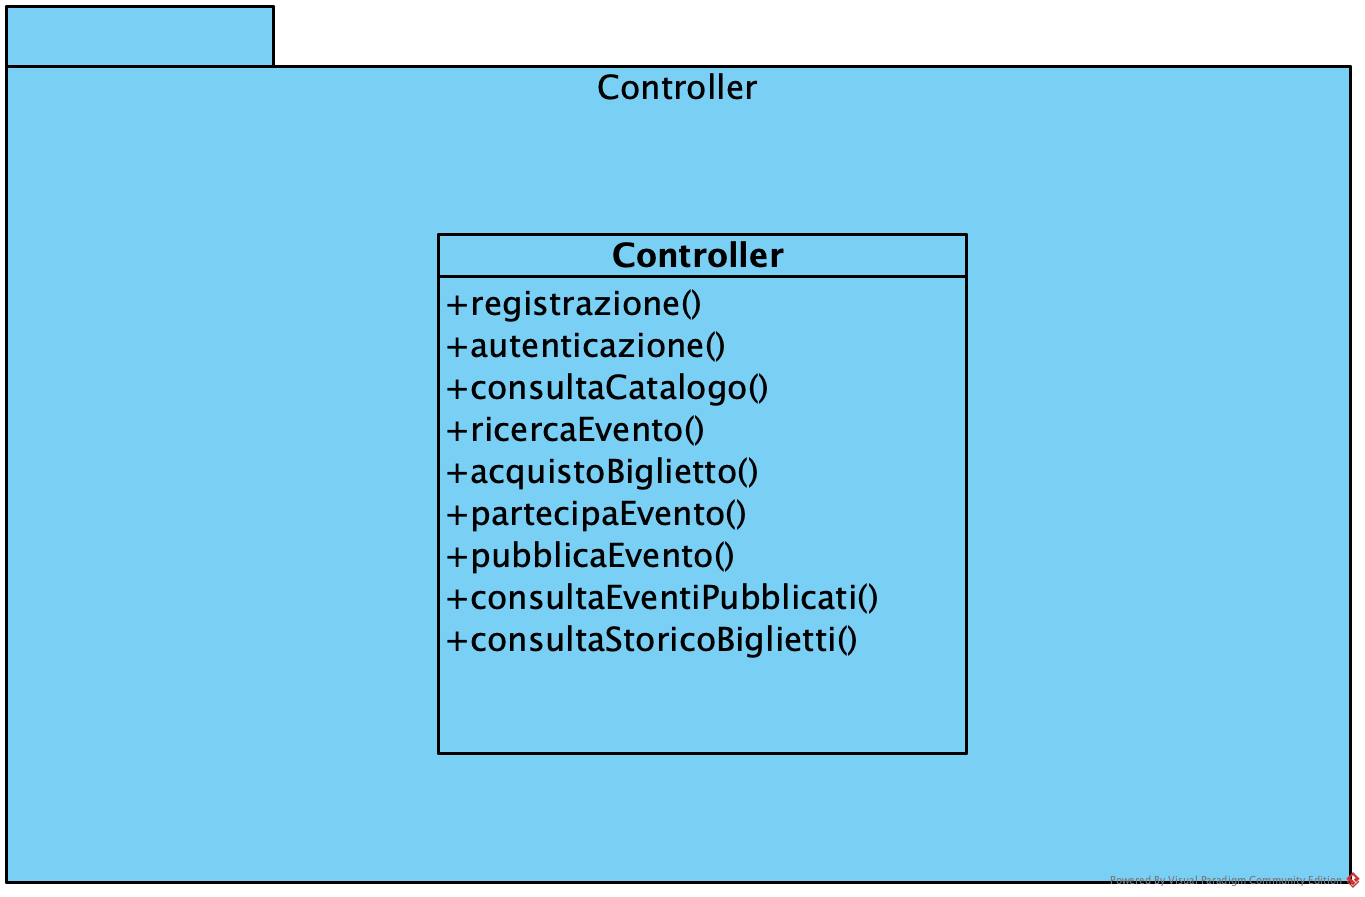
\includegraphics[height=0.38\linewidth]{assets/package/Controller.png}
	\vspace{1ex}
\end{center}
\subsection{Package Database}


\begin{center}	
	\vspace{1ex}
	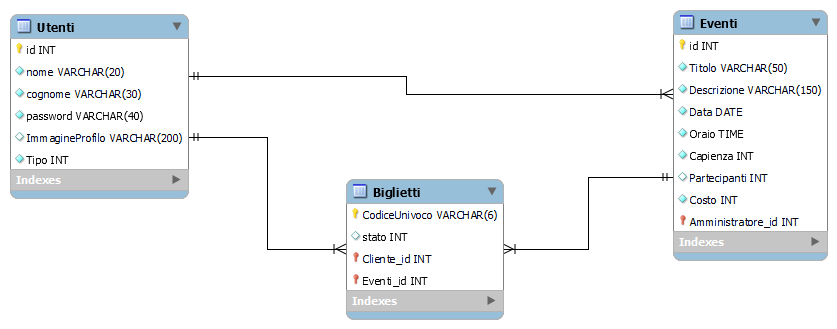
\includegraphics[height=0.38\linewidth]{assets/package/erdiagram.png}
	\vspace{1ex}
\end{center}

\begin{center}	
	\vspace{1ex}
	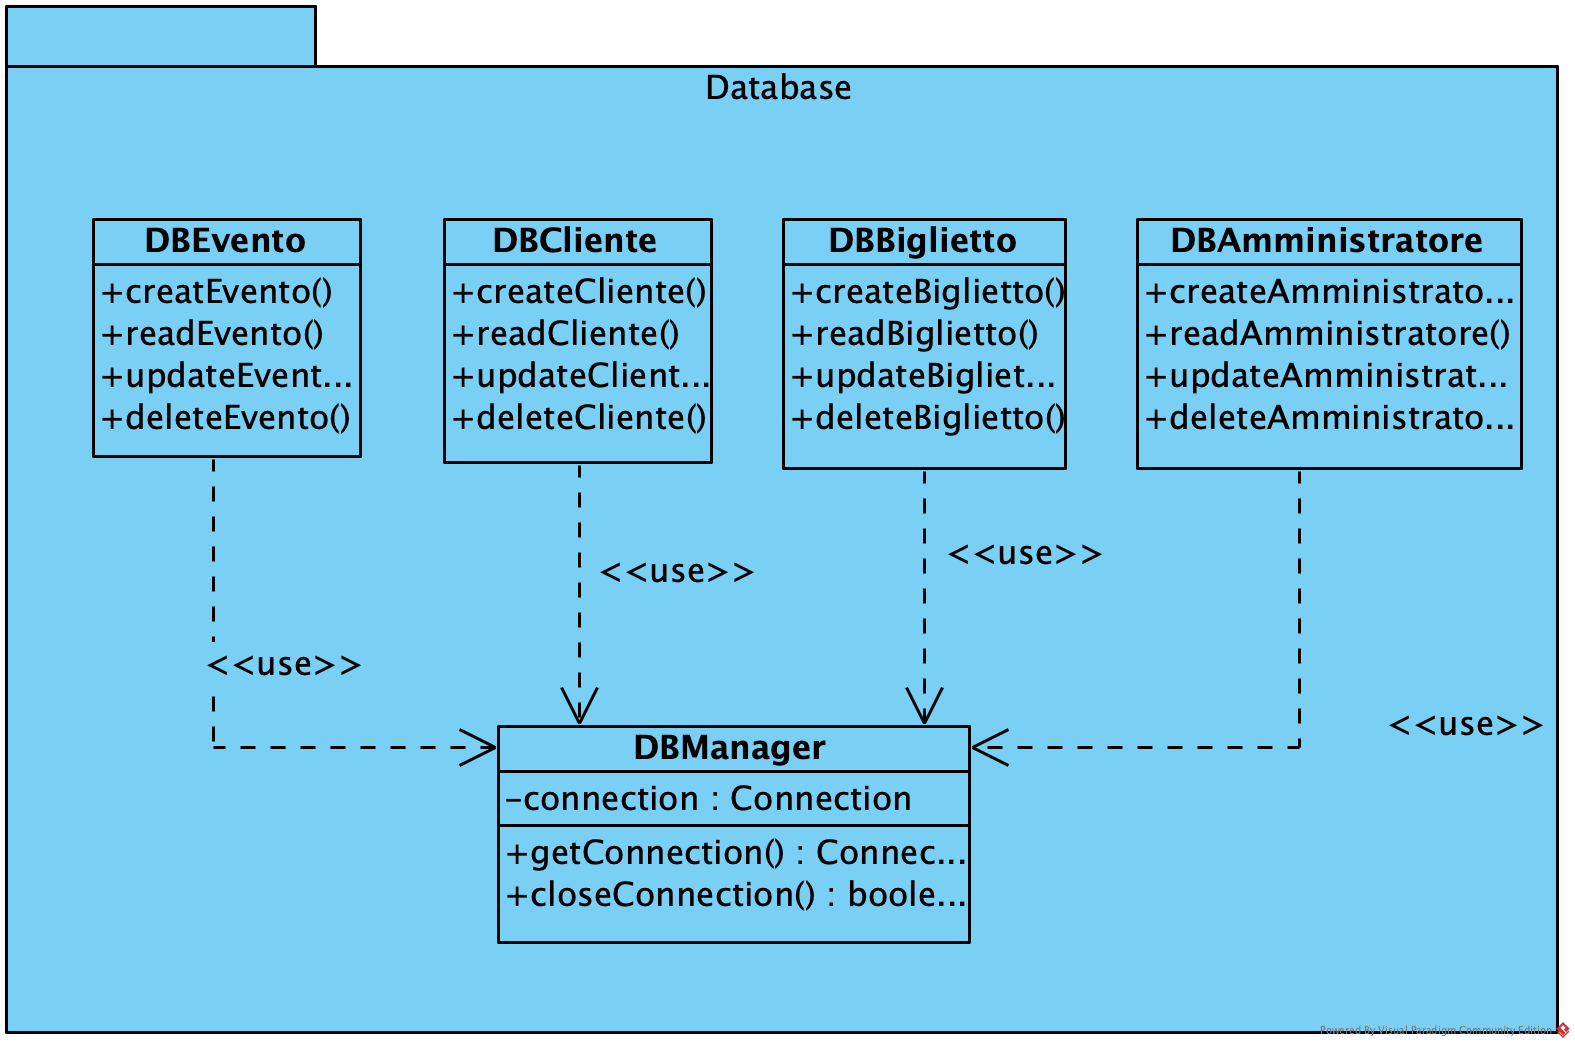
\includegraphics[height=0.38\linewidth]{assets/package/database1.png}
	\vspace{1ex}
\end{center}

Il modello E-R riportato rappresenta le principali entità e relazioni del sistema, progettato utilizzando MySQL Workbench.

In fase di progettazione si è scelto di rappresentare tutte e due i ruoli degli utenti all'interno di un'unica tabella denominata `Utente`. All'interno di questa tabella è stato inserito un attributo aggiuntivo, chiamato `Ruolo`, che consente di discriminare i due tipi di utente.

\section{Diagrammi di sequenza}
aspetto
